% 1998 上海文科第6题：工序流程图拓扑摹绘；边权以原卷标注为准，布局不按比例。
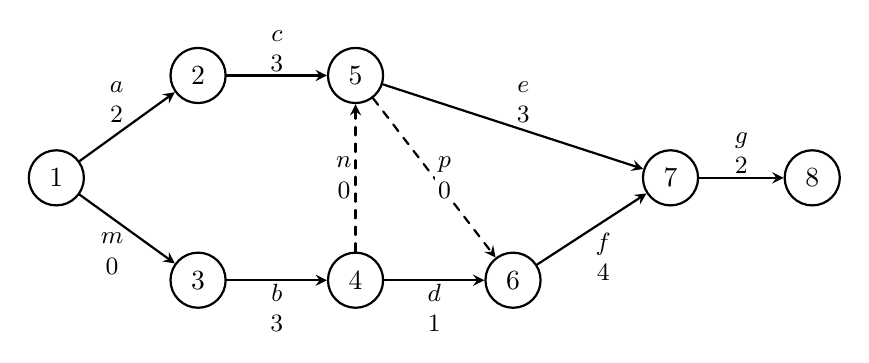
\begin{tikzpicture}[>=stealth,thick,line cap=round,line join=round,
  event/.style={circle,draw,minimum size=7mm,inner sep=0pt},
  activity/.style={font=\small,align=center,fill=white,inner sep=1pt}]
  \node[event] (v1) at (0,0) {1};
  \node[event] (v2) at (1.8,1.3) {2};
  \node[event] (v3) at (1.8,-1.3) {3};
  \node[event] (v4) at (3.8,-1.3) {4};
  \node[event] (v5) at (3.8,1.3) {5};
  \node[event] (v6) at (5.8,-1.3) {6};
  \node[event] (v7) at (7.8,0) {7};
  \node[event] (v8) at (9.6,0) {8};
  \draw[->] (v1) -- node[activity,above left] {$a$\\$2$} (v2);
  \draw[->] (v1) -- node[activity,below left] {$m$\\$0$} (v3);
  \draw[->] (v2) -- node[activity,above] {$c$\\$3$} (v5);
  \draw[->] (v3) -- node[activity,below] {$b$\\$3$} (v4);
  \draw[->,dashed] (v4) -- node[activity,left] {$n$\\$0$} (v5);
  \draw[->] (v4) -- node[activity,below] {$d$\\$1$} (v6);
  \draw[->,dashed] (v5) -- node[activity,right] {$p$\\$0$} (v6);
  \draw[->] (v5) -- node[activity,above right] {$e$\\$3$} (v7);
  \draw[->] (v6) -- node[activity,below right] {$f$\\$4$} (v7);
  \draw[->] (v7) -- node[activity,above] {$g$\\$2$} (v8);
\end{tikzpicture}
